\documentclass{article}
\usepackage[utf8]{inputenc}
\usepackage{graphicx}
\usepackage{multicol}
\usepackage{caption}
\usepackage{subcaption}
\usepackage{wrapfig}
\usepackage{float}
\usepackage{arydshln}
\usepackage{amsmath,amsthm,amssymb,amsfonts}
\usepackage{hyperref}
\usepackage{makecell}
\usepackage{listings}
\usepackage{epsfig}
\usepackage{color}
\usepackage{natbib}
\usepackage[table]{xcolor}
\usepackage[margin=1.1in]{geometry}
\usepackage[affil-it]{authblk}
\newtheorem{theorem}{Theorem}
\newtheorem{lemma}{Lemma}



\def\T{{\mathrm{\scriptscriptstyle T}}}
\def\bmath#1{\mbox{\boldmath$#1$}}

\bibpunct{(}{)}{;}{a}{}{,}
\setlength{\bibsep}{4.0pt}
\renewcommand{\baselinestretch}{1.1}


\title{\textbf{Some Title}}

\author{\vspace{11pt}Bridgette Delight}

\affil[1]{Department of Mathematics, Boise State University, Boise, Idaho 83725}
\affil[2]{Department of Computer Science, Boise State University, Boise, Idaho 83725}

\date{\today}


%------------------------------------------------------------------------------%
\begin{document}
%------------------------------------------------------------------------------%

\maketitle

\begin{abstract}

\end{abstract}

\vspace{8pt}
\noindent
KEY WORDS: Key word one; Key word two; Key word three; Key word four.

\section{Introduction}





\section{The Data}





\section{Methods}





\section{Results}



\begin{figure}[H]
    \centering
    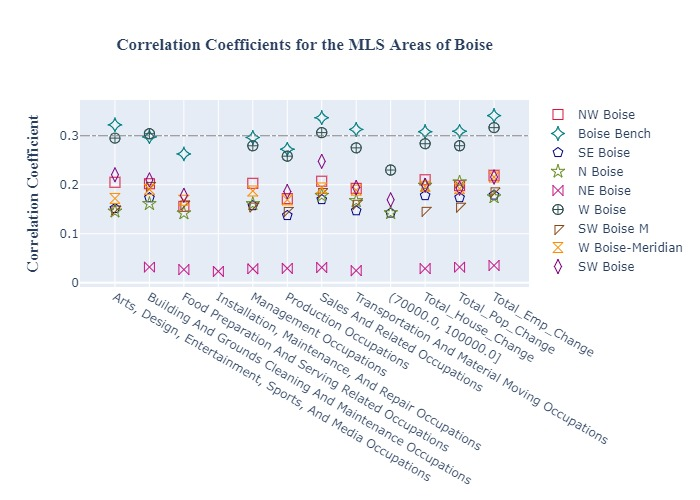
\includegraphics[width= .7\linewidth]{Area_fig.jpg}
    \caption{Caption}
    \label{fig: area_ccl}
\end{figure}

\begin{figure}
     \centering
     \begin{subfigure}[b]{0.45\textwidth}
         \centering
         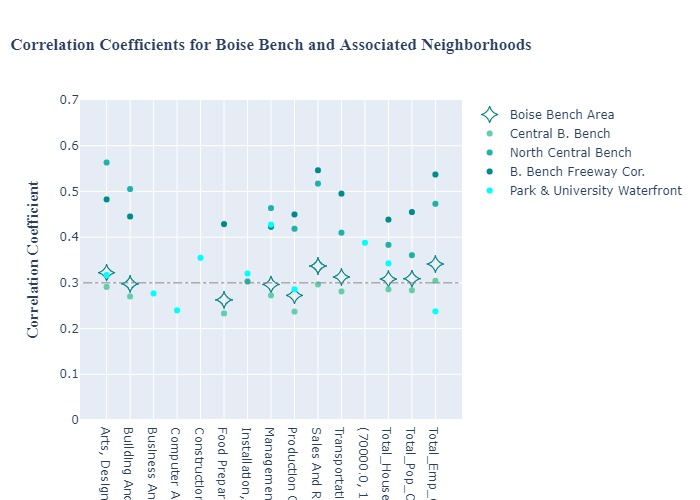
\includegraphics[width=\textwidth]{BB_fig.jpg}
         \caption{$y=x$}
         \label{fig:y equals x}
     \end{subfigure}
     \begin{subfigure}[b]{0.45\textwidth}
         \centering
         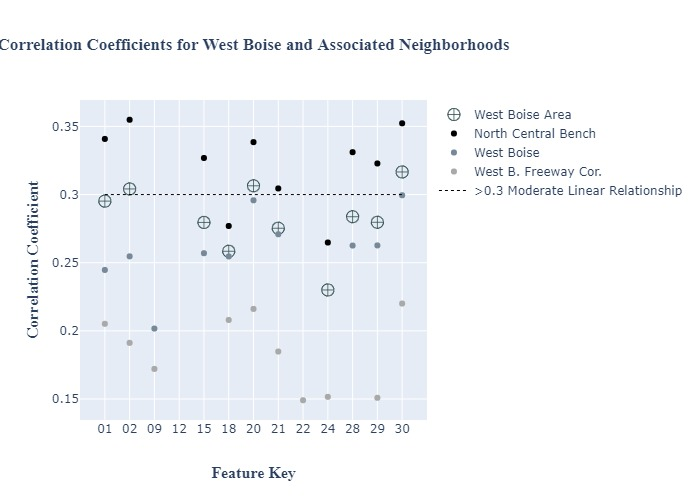
\includegraphics[width=\textwidth]{WB_fig.jpg}
         \caption{$y=3sinx$}
         \label{fig:three sin x}
     \end{subfigure}
          \begin{subfigure}[b]{0.45\textwidth}
         \centering
         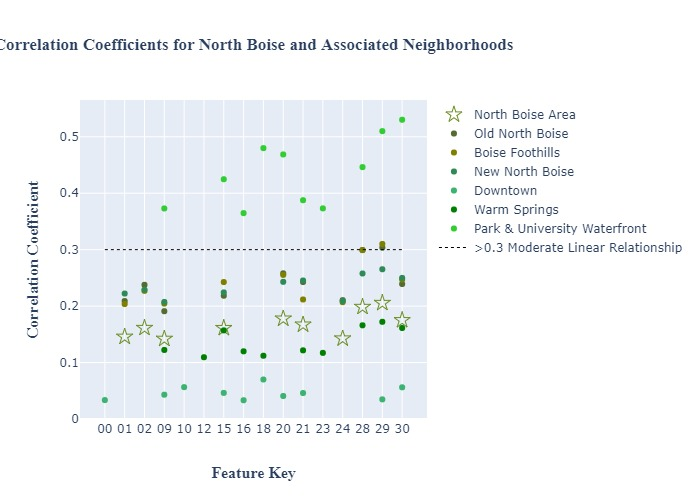
\includegraphics[width=\textwidth]{NB_fig.jpg}
         \caption{$y=3sinx$}
         \label{fig:three sin x}
     \end{subfigure}
          \begin{subfigure}[b]{0.45\textwidth}
         \centering
         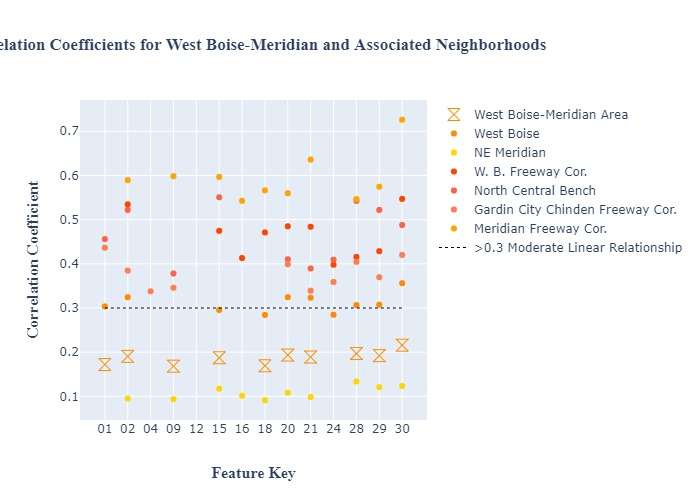
\includegraphics[width=\textwidth]{WBM_fig.jpg}
         \caption{$y=3sinx$}
         \label{fig:three sin x}
     \end{subfigure}
        \caption{Three simple graphs}
        \label{fig:three graphs}
\end{figure}


\section{Comments and Conclusions}



\appendix
\section{Appendix: Technical Details}



\section{Appendix: Code}

{\footnotesize
\begin{verbatim}
> ### Required packages
> library(car)                                               # required to use scatterplot()
> library(HH)                                                # required to use ci.plot()
>
> ### Read the dataset
> data.skin <- read.table(file=paste(WD.inp,"skincancer.txt",sep=""),header=TRUE)
> data.skin
\end{verbatim}
}

%------------------------------------------------------------------------------%
% References
%------------------------------------------------------------------------------%
\begin{thebibliography}{3}

\bibitem[\protect\astroncite{ACAO}{2019}]{ACAO:2019}
Ada County Assessor's Office (July 8, 2019)
\newblock \textit{Residential House Details for homes in Boise Idaho, from 2000-July 8, 2019}.
% Compiled by Alan Smith Strategic Development Analyst
%\newblock 


\bibitem[\protect\astroncite{KWR}{2019}]{KWR:2019}
Keller Williams Reality Boise (August 6, 2019)
\newblock \textit{Boise Neighborhood Guide}.
\newblock \url{https://www.weknowboise.com/boise-neighborhoods.php}


\bibitem[\protect\astroncite{BLS}{2019}]{BLS:2019}
United States Bureau of Labor Statistics (August 3, 2019)
\newblock \textit{Occupational Employment Statistics}.
% Last Modified Date: March 29, 2019
\newblock \url{https://www.bls.gov/oes/tables.htm}

\bibitem[\protect\astroncite{USC}{2019}]{ACAO:2019}
United States Census Bureau, Population Division (August 4, 2019)
\newblock \textit{Annual Estimates of Housing Units for the United States, Regions, Divisions, States, and Counties: April 1, 2010 to July 1, 2018 Release Date: May 2019}.
% https://factfinder.census.gov/faces/tableservices/jsf/pages/productview.xhtml?pid=PEP_2018_PEPANNHU&prodType=table
%\newblock \url{https://www.bls.gov/oes/tables.htm}
%https://www.census.gov/data/tables/time-series/demo/popest/intercensal-2000-2010-housing-units.html
%Suggested Citation: 


\bibitem[\protect\astroncite{Chen and Wu}{2008}]{Chen:Wu:2008}
Chen, J. and Wu, H. (2008)
\newblock Efficient local estimation for time-varying coefficients in
deterministic dynamic models with applications to {HIV}-1 dynamics.
\newblock \textit{Journal of the American Statistical Association}, 103, 369--384.

\bibitem[\protect\astroncite{Shumway and Stoffer}{2011}]{Shumway:Stoffer:2011}
Shumway, R. H. and Stoffer, D. S. (2011)
\newblock \textit{Time Series analysis and Its Applications With R Examples}, 3rd edn.
\newblock New York: Springer.
\end{thebibliography}
%-----------------------------------------------------------------------------%
\end{document}
%-----------------------------------------------------------------------------%
